\chapter{Diseño}

\section{SRD como afilador de flanco}
\label{sec:srd_sharpener}

En la sección \textcolor{red}{AGREGAR REF\ref{TODO}} fue explicado como un diodo
\textit{SRD} funciona como afilador de flanco.

En la figura \ref{fig:srd_sharpener} puede observarse un circuito que demuestra
el funcionamiento.

\begin{figure}
  \centering
    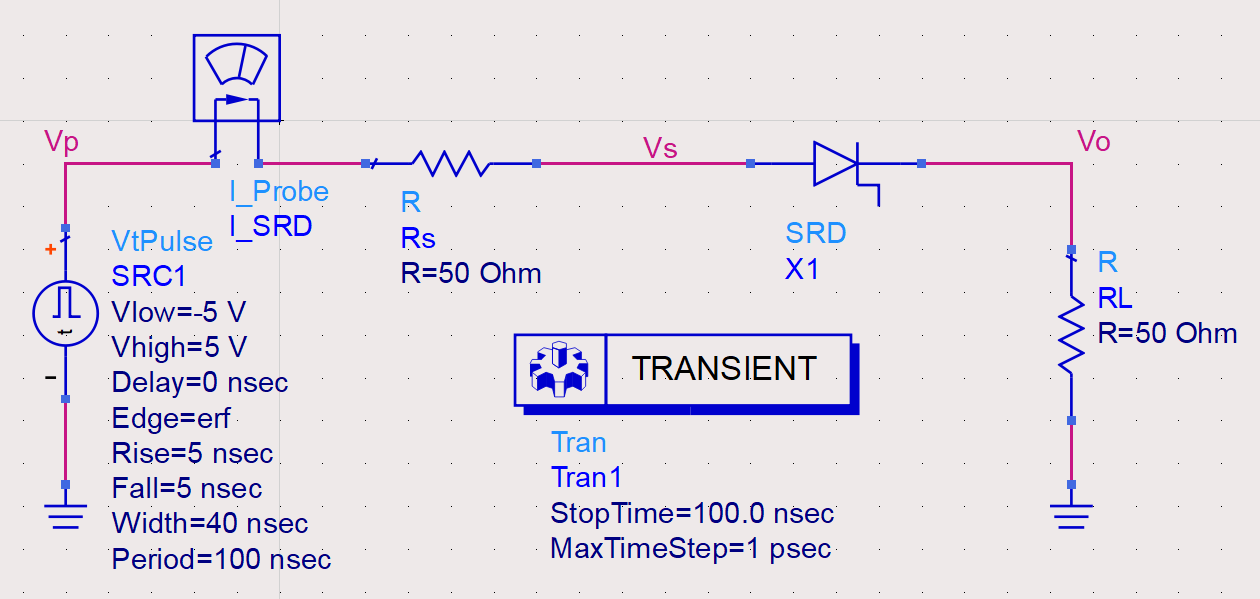
\includegraphics[width=0.6\textwidth]{images/srd_sharpener_circuit.png}
    \caption{Circuito afilador de flanco con SRD}
    \label{fig:srd_sharpener}
\end{figure}

El circuito está compuesto por un generador de cuadrada lento, con tiempos de
crecimiento y decrecimiento de \qty{5}{\nano\second}, en serie una resistencia
de fuente $R_s$ de valor \qty{50}{\ohm}. La carga del circuito es la resistencia
$R_L$ de \qty{50}{\ohm}.

\begin{figure}[tbp]
    \centering
    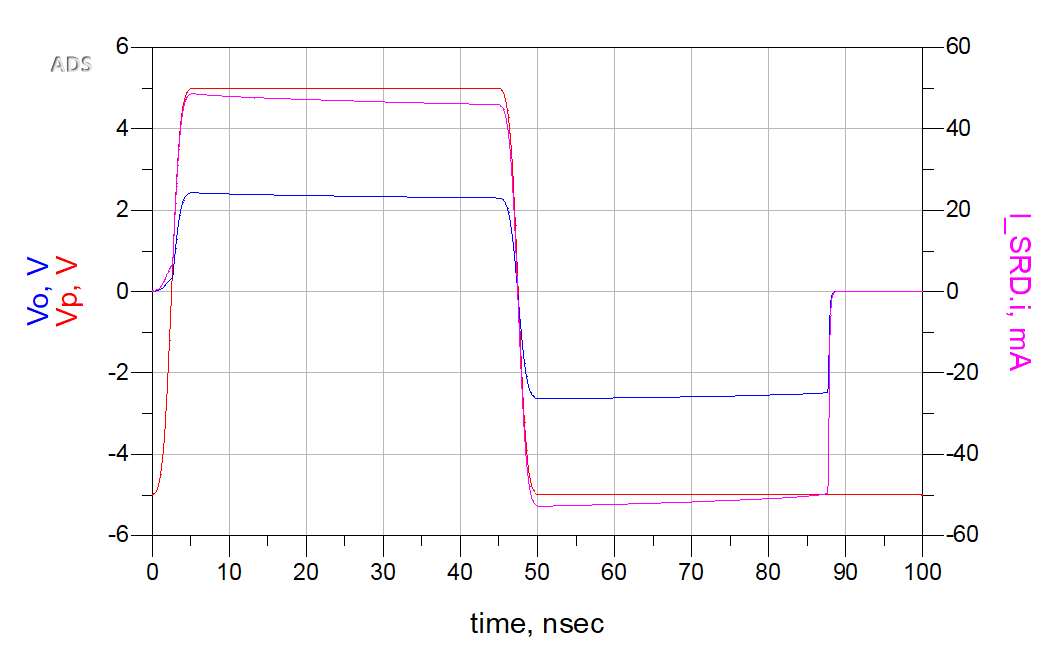
\includegraphics[width=0.8\textwidth]{images/srd_sharpener_result.png}
    \caption{Resultado de simulación.}
    \label{fig:srd_sharpener_result}
\end{figure}

En la figura \ref{fig:srd_sharpener_result} se observa el resultado de la
simulación. Vemos que, hasta aproximadamente \qty{85}{\nano\second}, la señal de
salida $V_o$ es igual a la señal de entrada, afectada por el divisor entre $R_L$
y $R_s$, $\frac{R_L}{R_L+R_s}$. Durante este tiempo, el \textit{SRD} presenta
una baja impedancia. En la porción positiva de la señal de entrada $V_p$, esto
es coincidente con un diodo usual, ya que el mismo se encuentra polarizado en
directa. En lo que destaca el \textit{SRD} de un diodo usual, es que luego de que la
tensión de entrada se invierta, este sigue presentando una baja impedancia. Esto
se debe al gran tiempo de vida de sus portadores minoritarios, lo que requiere
un tiempo apreciable para descargarlos y pasar al estado de alta impedancia.

Se observa en la forma de onda de $V_o$ que esta transición se da alrededor de
\qty{85}{\nano\second}, done la tensión de salida cae abruptamente a $0$. En la
figura \ref{fig:srd_sharpener_result} puede observarse el comportamiento
de la corriente. Se observa la misma caída abrupta en los
\qty{85}{\nano\second}, y una inversión en el signo de la corriente con la
inversión en el signo de la cuadrada de entrada.

\begin{figure}[tbp]
    \centering
    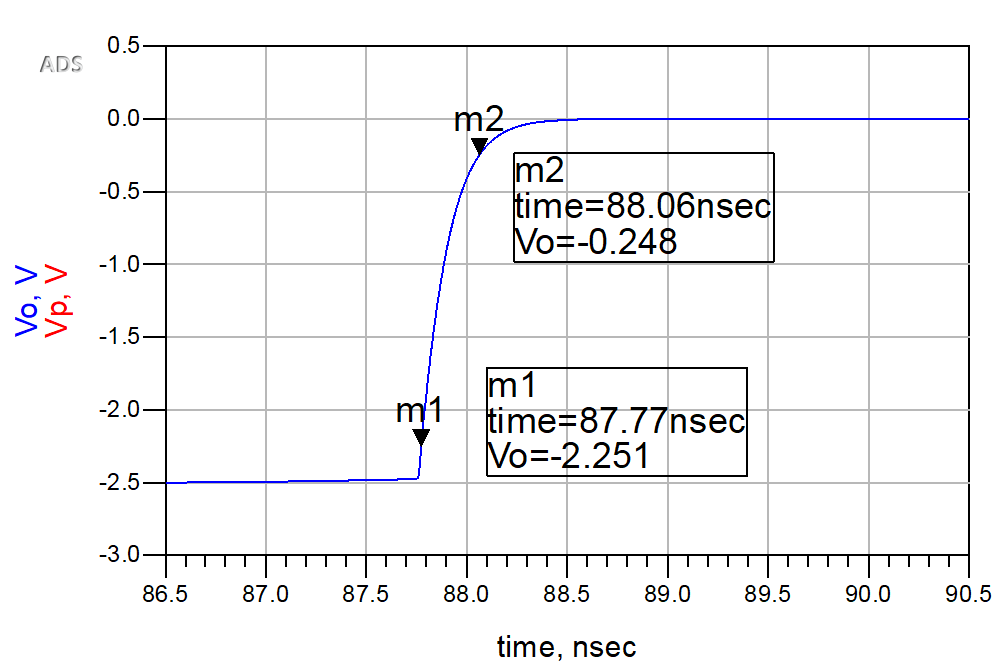
\includegraphics[width=0.8\textwidth]{images/srd_sharpener_result_rise_time.png}
    \caption{Tiempo de crecimiento.}
    \label{fig:srd_sharpener_result_rise_time}
\end{figure}

Llamaremos corriente de inyección de carga $I_F$ a la corriente que circula por
el \textit{SRD} con sentido positivo. Esta corriente determina la carga
almacenada en el mismo, y ambas se relacionan mediante \cite{an918},
\cite{moll1969}

\begin{equation}
    Q_F = I_F \cdot \tau \cdot \left( 1 - e^{-t_F/\tau}\right)
\end{equation}

Para el circuito presentado, la corriente $I_F$ estará dada por

\begin{equation}
    I_{F} = \frac{V_h}{R_s+R_L}
\end{equation}

con $V_h$ el valor de la tensión positiva de la señal cuadrada de entrada.

Para la corriente de extracción de carga $I_R$, que es la corriente que extrae
carga durante el tiempo en el que el \textit{SRD} se encuentra en un estado de
baja impedancia y la corriente que circula es negativa, tenemos la siguiente
expresión

\begin{equation}
    I_{R} = \frac{V_l}{R_s+R_L}
\end{equation}

con $V_l$ el valor de la tensión negativa de la señal cuadrada de entrada.

En la figura \ref{fig:srd_sharpener_result_rise_time}, puede observarse el
tiempo de crecimiento del escalón generado con el apagado del \textit{SRD}. Se
toma el tiempo de crecimiento \qty{10}{\percent}-\qty{90}{\percent}. Siendo que
el escalón de tensión se da entre \qty{-2.5}{\volt} y \qty{0}{\volt}, tenemos
que el punto de \qty{10}{\percent} es $V_{10\%} = -2.5 \ V \ \cdot 0.9 =  2.25 \
V$, y el de \qty{90}{\percent} es $V_{90\%} = -2.5 \ V \ \cdot 0.1 =  -0.25 \
V$.

En cuanto a la magnitud del salto de tensión $\Delta V$, estará dado por el
valor de la tensión en el cátodo del \textit{SRD} antes de que pase al estado de
alta impedancia. Esta tensión estará dada por el divisor entre $R_L$ y $R_s$,

\begin{equation}
    \Delta V = V_l \cdot \frac{R_L}{R_L+R_s}
\end{equation}

El tiempo de crecimiento de este escalón estará dado por dos componentes: un
tiempo de transición del diodo SRD $t_t$, y un tiempo de carga $RC$ dado por el
tiempo en que demora en cargarse el RC. \textcolor{red}{COMPLETAR CON EXPRESIÓN}
\cite{an918}.

\textcolor{red}{EXPLICAR IMPORTANCIA DE BAJA CAPACIDAD PARALELO AL SRD}

Vemos por los marcadores de la figura, que estos tiempos son
\qty{87.77}{\nano\second} y \qty{88.06}{\nano\second} respectivamente, por lo
que tenemos un tiempo de crecimiento

\begin{equation}
    t_r = \qty{87.77}{\nano\second} - \qty{88.06}{\nano\second} =
    \qty{290}{\pico\second}
\end{equation}

Como fuese explicado en la sección \textcolor{red}{AGREGAR REF\ref{TODO}}, este
tiempo de crecimiento estará dado por el tiempo de transición del diodo y por el
tiempo del RC formado entre la capacidad de reversa del diodo y la resistencia
vista desde los nodos del capacitor.

\section{Generador de pulsos con \textit{stub}}

\subsection{Principios del \textit{stub}}

Un \textit{stub} consiste de una línea de transmsión conectada en paralelo al
camino de la señal. Su efecto sobre la señal dependerá de su impedancia
característica, largo e impedancia de terminación \cite{pozar2011}.

Cuando el \textit{stub} se encuentra abierto, es decir, terminado por una
impedancia infinita, la señal propagada se verá reflejada con signo positivo, y
en el caso de una línea de transmisión sin pérdidas, con un factor de ganancia
unitario. En el caso de una línea de transmisión real, las pérdidas resultaran
en un factor de atenuación. \textcolor{red}{chequear esto de la atenuación, y lo
q sigue de las aplicaciones de un stub abierto}.  Este efecto permite generar
resonancias en ciertas frecuencias, útiles para filtrado de señales o adaptación
de impedancias.

En el caso de un \textit{stub} cortocircuitado, es decir, con una impedancia de
terminación igual a $0$, el efecto será una reflexión de la señal con fase
opuesta, y un factor de atenuación dado por las pérdidas de la línea.

El caso de interés para el circuito generador de pulsos, es el del \textit{stub}
cortocircuitado, ya que la reflexión de señal con fase opuesta, permite generar
un pulso en base a una forma de onda creciente o decreciente.

\begin{figure}[tbp]
    \centering
    
\includegraphics[width=0.8\textwidth]{images/placeholder.jpg}
    \caption{Reflexiones en un \textit{stub} cortocircuitado.}
    \label{fig:images-placeholder-jpg}
\end{figure}

En la figura \ref{TODO figura con funcionamiento temporal del stub} se observa
el principio de funcionamiento. Se observa un pulso de entrada, formado por una
forma de onda de tipo escalón, en nuestro caso este escalón será el mismo que en
la figura \ref{srd_sharpener_result_rise_time}. Este escalón se ve reflejado con
polaridad opuesta, y se suma al escalón de entrada.

Dado el tiempo de propagación de la línea de transmisión $T$, vemos que el
tiempo que tarda el pulso de entrada en reflejarse es $2*T$, el tiempo de un
camino de ida y vuelta. Dado que el pulso se forma cuando vuelve la componente
reflejada, vemos que el ancho de pulso estará dado por $2*T$. De esta forma, la
duración temporal del pulso y, por lo tanto, el ancho de banda del sistema,
estará dado por la longitud $L$ del \textit{stub}.

El tiempo de propagación $T$ está dado por la velocidad de propagación en la
línea de transmisión $v_p$ y el largo de la línea $L$. La velocidad de
propagación está dada por \textcolor{red}{AGREGAR REF, POZAR?} \cite{pozar2011}

\begin{equation}
  v_p = \frac{c_0}{\sqrt{\kappa}}
\end{equation}

con $\kappa$  la permitividad relativa del medio. Para una línea de transmisión,
es posible desarrollar una \textit{permitividad relativa efectiva}, que es una
función de la geometría de la línea y sus materiales \cite{pozar2011}. Esta
función puede obtenerse a través de una forma cerrada, generalmente involucrando
diversas aproximaciones, o mediante métodos numéricos iterativos. El punto a
resaltar es que, dada una determinada estructura de línea de transmisión y sus
materiales, se puede considerar a $\kappa$ una constante del circuito.

Es interesante notar que $\kappa$ es una función del corte transversal de la
línea de transmisión, y no de su dimensión longitudinal. De esta manera,
$\kappa$ es independiente del largo $L$ de la línea \cite{pozar2011}.

Entonces, el ancho de pulso $T_p$ está dado por

\begin{equation}
  T_p = 2*T = 2*v_p*L =2*\frac{c_0}{\sqrt{\kappa}}*L
\end{equation}

De esta forma, se puede diseñar el largo de línea $L$ para obtener un ancho de
pulso $T_p$ deseado

\begin{equation}
  L = \frac{T_p}{2}\frac{\sqrt{\kappa}}{c_0}
\end{equation}

De esta manera, el largo $L$ queda determinado por el ancho de pulso deseado
$T_p$ y la constante de propagación de la línea de transmisión utilizada
$\kappa$.

\subsection{Generador de pulsos SRD+\textit{stub}}

Agregando un \textit{stub} cortocircuitado al afilador de flancos SRD
descripto anteriormente, podemos formar un generador de pulsos ultracortos. El
SRD genera un flanco rápido, y este flanco es convertido en un pulso
mediante la reflexión con fase opuesta en el \textit{stub}. 

El ancho de pulso es controlado por el largo del \textit{stub} como fuese
explicado anteriormente. La amplitud por la amplitud de la fuente, la relación
entra la impedancia de carga $Z_L$ y la del generador $Z_g$ y por el largo del
stub.

Como fuese explicado en secciones anteriores \textcolor{red}{EXPLICAR EN QUÉ
SECCIÓN}, el escalón de tensión generado en el SRD tiene una magnitud dada por

\begin{equation}
    \Delta V = V_l \cdot \frac{R_L}{R_L+R_s}
\end{equation}

El ancho del pulso, estará dado por el valor de este escalón en el instante en
el que el pulso reflejado se recombina, como puede observarse en la figura
\textcolor{red}{FIGURA MOSTRANDO REFLEXIÓN STUB}. Si asumimos que el escalón
crece como un sistema de primer orden con constante de tiempo $\tau$, el valor
del escalón en función del tiempo es

\begin{equation}
  V(t) = \Delta V \left( 1-e^{-\frac{t}{\tau}}\right)
\end{equation}

Siendo el tiempo que tarda el pulso en reflejarse ida y vuelta $2T$ o $T_p$, la
amplitud del pulso estará dada por

\begin{equation}
    \label{eq:A_p}
    A_p = V(2T) = V_l \cdot \frac{R_L}{R_L+R_s} \left( 1-e^{-\frac{2T}{\tau}}\right)
\end{equation}

Vemos que $\Delta V$ es el máximo valor que puede alcanzar el pulso, siendo la
relación $\frac{2T}{\tau}$ la que determina que porcentaje de este valor tomará
el pulso. Para $ \tau \ll T $, será $e^{-\frac{2T}{\tau}} \approx 1$, y por lo
tanto $A_p \approx 0$. Este es el mismo resultado que intuitivamente se
obtendría, que para señales con una variación temporal $\tau$ mucho menor al
tiempo de propagación en el \textit{stub} $T$, la señal será filtrada por el
efecto de puesto a tierra.

Para el caso de la señal de escalón generada por el SRD, es fácil obtener un
tiempo de crecimiento del orden de los cientos de picosegundos, por lo que su
amplitud resulta un porcentaje considerable de $\Delta V$. Cuanto más rápido sea
el flanco, mayor amplitud.

En la figura \ref{fig:stub_generator_circuit} podemos observar un esquemático
del generador de pulsos basado en SRD y \textit{stub}. La fuente es simétrica,
con amplitudes de \qty{\pm 5}{\volt}. La impedancia de fuente $Z_g$ se encuentra
perfectamente adaptada a la de carga $Z_L$, siendo ambas de \qty{50}{\ohm}. La
línea de transmisión es ideal, caracterizada únicamente por su impedancia
característica, \qty{50}{\ohm} en este caso, y su retardo de propagación,
\qty{60}{\pico\second} en este caso.

\begin{figure}[tbp]
    \centering
    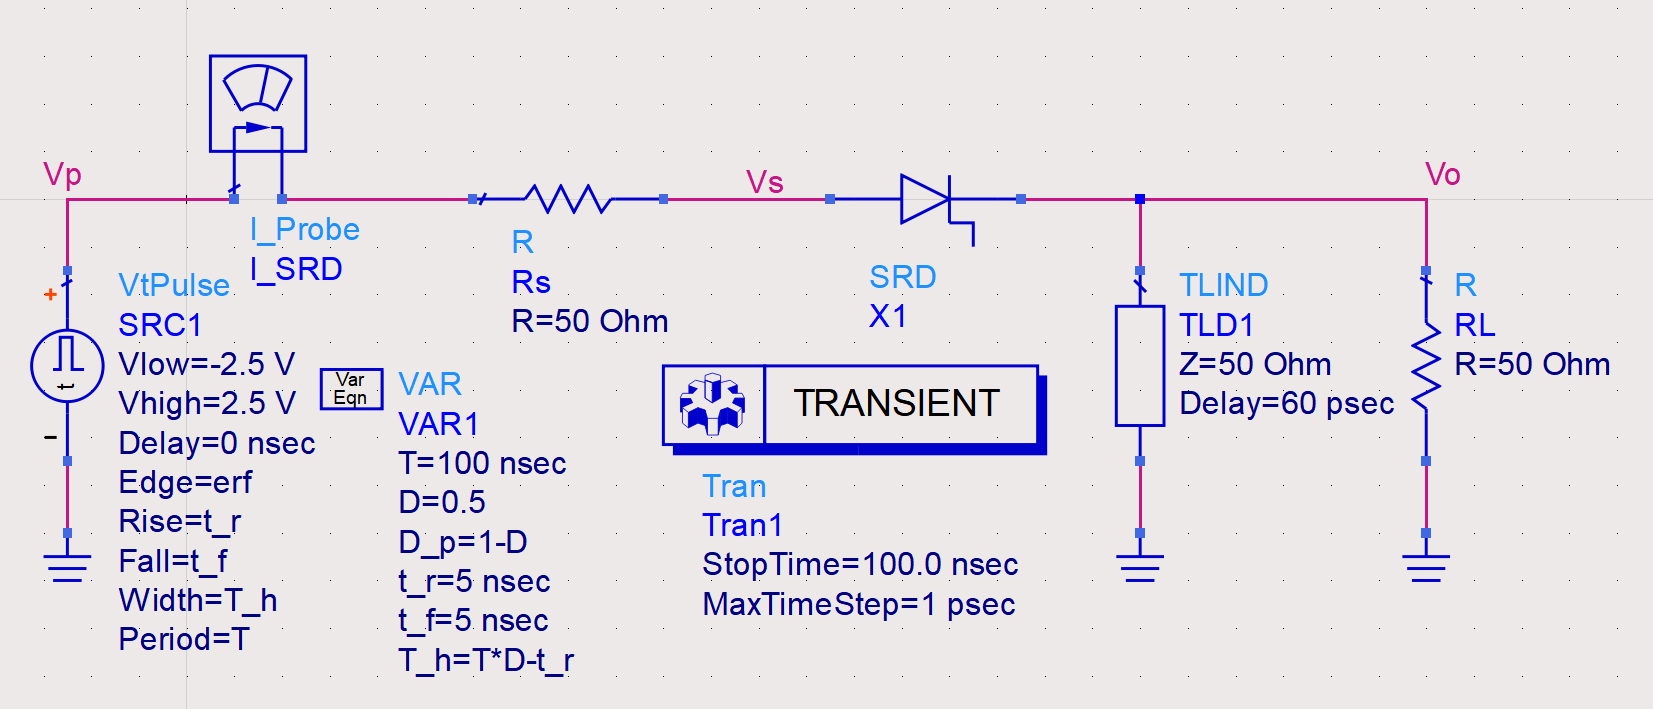
\includegraphics[width=0.8\textwidth]{images/stub_generator_circuit.png}
    \caption{Generador de pulsos basado en \textit{stub}}
    \label{fig:stub_generator_circuit}
\end{figure}

En las figuras \ref{fig:generator_result_waves} y
\ref{fig:stub_generator_result_pulse} se observan los resultados de la
simulación del esquemático de la figura \ref{fig:stub_generator_circuit}. En la
figura \ref{fig:generator_result_waves} se observan las formas de onda de la
señal de entrada $V_p$, la tensión de salida $V_o$ y la corriente sobre el SRD
$I_{SRD}$. Se observa que la tensión de salida $V_o$ sigue a la de entrada $V_p$
hasta aproximadamente \qty{85}{\nano\second}, donde el SRD pasa del estado de
baja impedancia al de alta. En en este instante, se forma un pulso por una
combinación del salto de tensión en el SRD y el efecto de reflexión del stub
cortocircuitado. Es interesante notar que los flancos positivos y negativos de
la señal de entrada también resultan en pulsos a la salida, aunque de mucha
menor amplitud. La forma de onda de la corriente es coincidente con lo
mencionado anteriormente, siendo una versión escalada por la impedancia de la
forma de onda de entrada $V_p$, hasta los \qty{85}{\nano\second}, donde cae
abruptamente a $0$ debido al cambio de impedancia en el SRD.

Es interesante notar que en este caso, los valores de la corriente están dados
por $\frac{V_p}{R_s}$ y no $\frac{V_p}{R_s+R_L}$ como en la sección
\ref{sec:srd_sharpener}. Esto se debe a que el \textit{stub} actua como un
cortocircuito sobre $R_L$, anulando su impedancia. Es importante notar que,
entonces, $R_S$ tiene la función de limitación de corriente durante las etapas
de conducción del SRD. De ser $0$ esta impedancia, la corriente sería infinita
(en rigor, se vería limitada únicamente por la resistencia serie del SRD)

En la figura \ref{fig:stub_generator_result_pulse} se observa un zoom sobre el
pulso obtenido. Tiene una amplitud de \qty{1.728}{\volt}, y una duración
de \qty{180}{\pico\second} \textcolor{red}{por qué no es 60*2=120?}
\textcolor{red}{verificar que la amplitud coincida con la expresión anterior}.
Se observa que el pulso presenta un sobretiro negativo, una no idealidad no
contemplada hasta ahora en el modelo presentado.

\textcolor{red}{Hablar sobre la falta de reflexiones en el stub por ser de 50
ohm, q es la impedancia q ve una vez q se abre el SRD? ver q pasa si movemos esa
Zo?}

\begin{figure}[tbp]
    \centering
    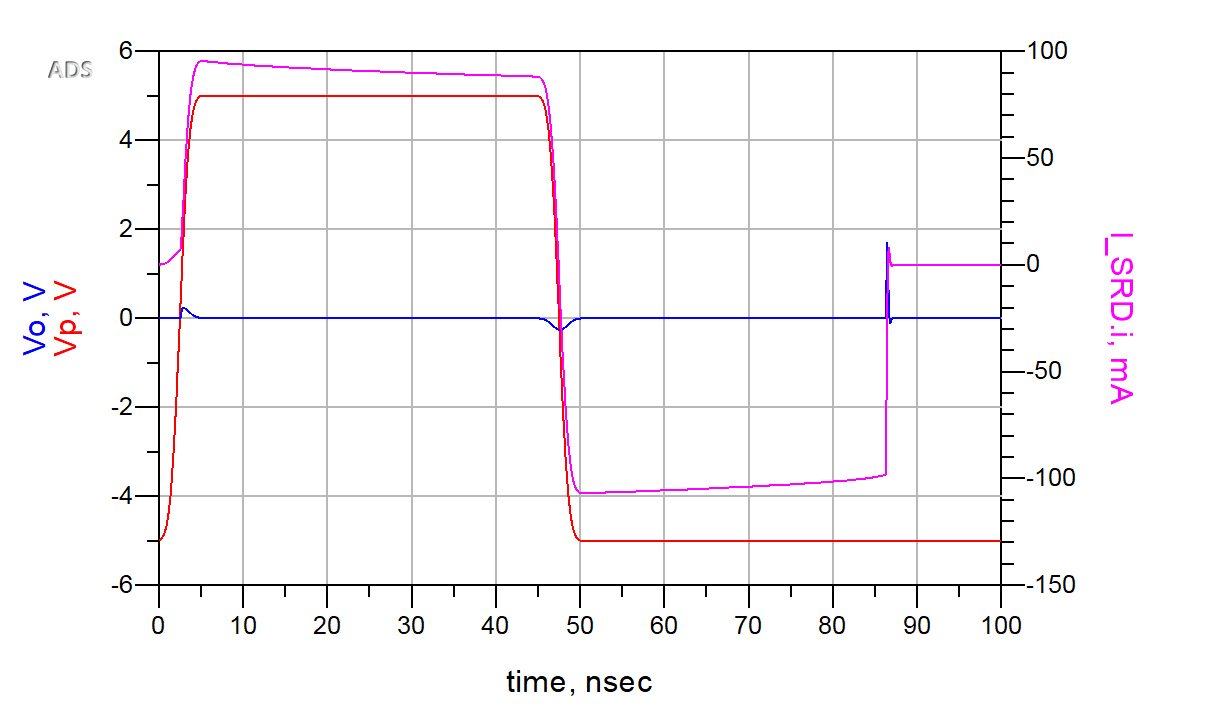
\includegraphics[width=0.8\textwidth]{images/stub_generator_result_waves.png}
    \caption{Resultado de simulación de generador con \textit{stub}}
    \label{fig:generator_result_waves}
\end{figure}

\begin{figure}[tbp]
    \centering
    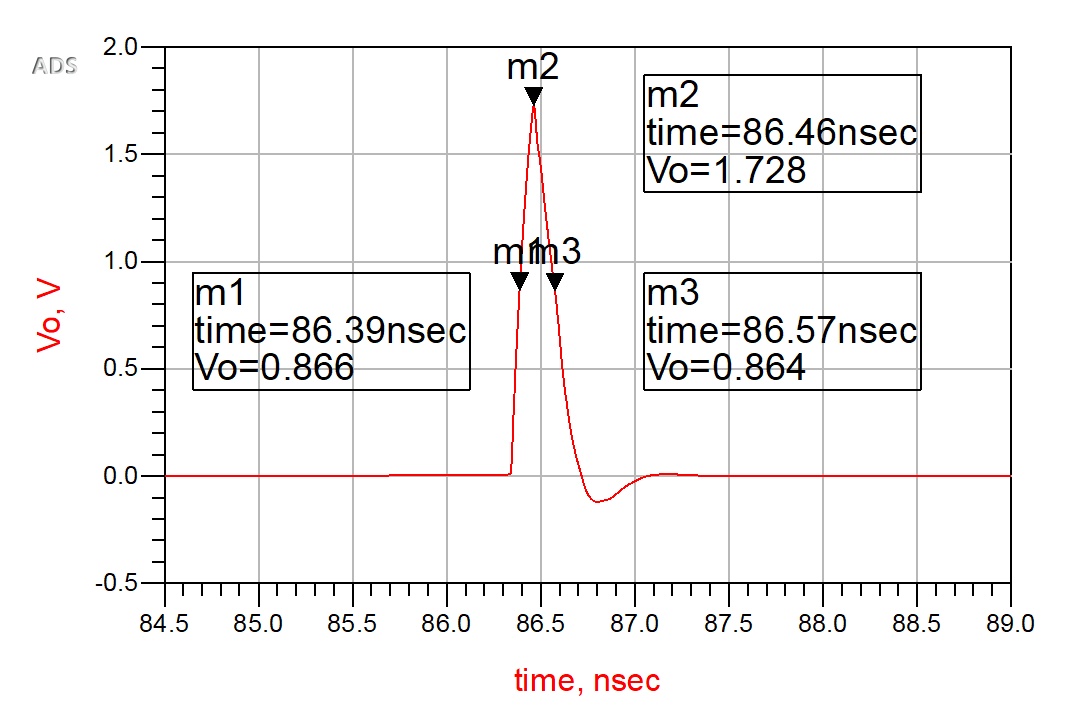
\includegraphics[width=0.8\textwidth]{images/stub_generator_result_pulse.png}
    \caption{Pulso simulado con generador con \textit{stub}}
    \label{fig:stub_generator_result_pulse}
\end{figure}

\subsection{Diseño del \textit{stub}}

En algún lado cómo obtuvimos el largo en mm del stub.

\section{Diseño final del \textit{pulser}}

\textcolor{red}{mostrar oscilaciones en el resultado anterior para justificar la
inclusión del Schottky}

Para compensar tanto las transmisiones de los flancos de la fuente de entrada y
el sobretiro negativo observado, se agrega al generador un diodo rectificador en
serie con la resistencia de carga $R_L$. Siendo la tensión de encendido del
diodo mayor a la amplitud de los pulsos generados por las transiciones de la
onda de entrada, estos no serán transmitidos a la carga $R_L$ debido a la acción
de rectificación. En cuanto al sobretiro y las oscilaciones, tampoco serán
transmitidas a la salida debido al bloqueo de de corriente en sentido negativo.

El costo de este diodo es la perdida de amplitud en el pulso principal, dada por la
magnitud de su tensión de encendido. Para un correcto funcionamiento del
generador de pulsos, es fundamental que el rectificador sea lo suficientemente
rápido como para transmitir el pulso ultracorto sin degradación. Por esta razón
se utiliza un diodo Schottky.

\subsection{Selección del diodo}

Se utilizó un \textcolor{red}{MAE...}. Este posee una baja capacidad. Hablar del
pequeño factor de forma.

\subsection{Simulaciones}

En la figura \ref{fig:pulser_final_schematic} se observa un esquemático del
generador de pulsos con el rectificador incluido. En la figura
\ref{fig:generator_schottky_result_waves} se observa el resultado de la
simulación. Para este caso, en la salida se encuentra únicamente el pulso
principal, habiéndose anulados los pulsos generados por las transiciones de la
señal de entrada.

En la figura \ref{fig:schottky_generator_result_pulse} se observa el pulso
simulado. Con respecto al de la simulación sin rectificador, figura
\ref{fig:stub_generator_result_pulse}, se observa una caída en la amplitud de
\textcolor{red}{COMPLETAR VALOR}, dada por la tensión de encendido del Schottky
utilizado, y una reducción del sobretiro y las oscilaciones
\textcolor{red}{MOSTRAR QUE ESTO SE REDUCE}.

\begin{figure}[tbp]
    \centering
    
\includegraphics[width=0.8\textwidth]{images/placeholder.jpg}
    \caption{\textit{Pulser} final incluyendo diodo Schottky}
    \label{fig:pulser_final_schematic}
\end{figure}

\begin{figure}[tbp]
    \centering
    
\includegraphics[width=0.8\textwidth]{images/placeholder.jpg}
    \caption{Resultado de simulación de generador con rectificador}
    \label{fig:generator_schottky_result_waves}
\end{figure}

\begin{figure}[tbp]
    \centering
    
\includegraphics[width=0.8\textwidth]{images/placeholder.jpg}
    \caption{Pulso simulado con generador con rectificador}
    \label{fig:schottky_generator_result_pulse}
\end{figure}

\section{Consumo del generador}

Cálculos de cuánto consume el generador, cuanto disipan los componentes.

\section{Diseño del \textit{driver}}

\section{Arquitectura}

Dado que uno de los objetivos del trabajo es un generador de pulsos que pueda
ser controlado por la salida digital de un sistema embebido, y dado que estas
salidas son en la mayoría de los casos unipolares y de baja capacidad de carga,
es necesario incluir en el prototipo una etapa \textit{driver}.

La función de esta etapa es, en base a un pulso digital de entrada de control, y
una fuente de alimentación continua, generar el pulso bipolar necesario para el
funcionamiento del \textit{pulser}. Este pulso bipolar tendrá un ciclo de
trabajo y un período dados por el ciclo de trabajo y el período del pulso
unipolar de entrada. Es necesario también que el \textit{driver} presente una
baja carga al pulso unipolar.

En la figura \ref{fig:driver_block_diagram} se observa un diagrama en bloques
del driver propuesto. El mismo está compuesto por dos componentes principales
que brindan dos funciones diferenciadas, la llave y el capacitor. A la entrada
es excitado por la señal digital de control, y a la salida tiene una carga
$Z_L$. La carga en este caso será el pulser, por lo tanto será una carga no
lineal, ya que como se mostro en secciones anteriores, la corriente que consume
tiene una abrupta caída a 0 cuando se abre el SRD.

\begin{figure}[tbp]
    \centering
    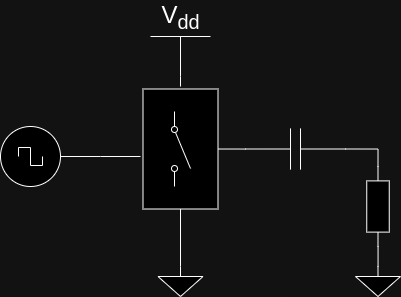
\includegraphics[width=0.8\textwidth]{images/driver.drawio.png}
    \caption{Diagrama en bloques del driver}
    \label{fig:driver_block_diagram}
\end{figure}

\subsection{Llave}

La llave conmuta entre $V_{dd}$ y tierra según la señal de control digital. De
esta manera, la corriente que consume la carga es entregada por la fuente y no
por la señal de control digital. A la salida de la llave se generará una señal
cuadrada unipolar, pero a diferencia de la entrada, esta conmutará entre
$V_{dd}$ y tierra, mientras que a la entrada se conmuta entre $V_{dig}$ y
tierra. De esta manera, la llave logra presentarle una carga baja y constante a
la salida digital, y amplifica la conmutación a todo el rango disponible con la
fuente de alimentación. Esta es una aproximación ideal, en realidad será todo el
rango de la fuente de alimentación menos la caída que tenga el bloque.

A la salida de la llave tenemos entonces una señal cuadrada unipolar, con
amplitud pico a pico igual a $V_{dd}$, es decir, toda la amplitud disponible de
la fuente de alimentación, y una capacidad de entrega de corriente considerable.

\subsection{Filtro pasa altos}

Sabemos que un pulso cuadrado unipolar de período $T$ tendrá un espectro dado
por una componente de continua con el valor medio $V_{m}$, y múltiples
harmónicos de $T$, cada uno con una amplitud que decae con $\frac{1}{n}$.
\textcolor{red}{agregar una referencia que banque esto}.

Entonces, podemos pensar al pulso unipolar como la suma de un pulso bipolar de
valor medio 0, y una constante con valor igual al valor medio del pulso
unipolar. Entonces, podemos obtener al pulso bipolar restándole al unipolar su
valor medio.

Teniendo en cuenta que el valor medio es la componente de DC del pulso, podemos
lograr este resultado pasando el pulso unipolar por un filtro pasaltos. El ancho
de banda de este filtro debe ser tal que filtre la componente de continua y no
distorsione las componentes alternas, que se encuentran a partir de $T$.

Sabemos que un filtro pasa altos de primer orden con frecuencia de corte $f_c$
tiene una característica de magnitud que presenta atenuación desde continua hasta
aproximadamente $f_c$, y una fase que varía \qty{90}{\degree} desde
$\frac{f_c}{10}$ hasta $f_c \cdot 10$. Entonces, para filtrar la componente
continua de la unipolar y transmitir la bipolar sin distorsión,
es necesario que la frecuencia de la cuadrada sea mayor a 10 veces $f_c$, es
decir $T > 10 \cdot f_c$, o $f_c < \frac{T}{10}$

Siendo la $PRF$ objetivo de \qty{10}{\mega\hertz}, el requerimiento sobre $f_c$
es entonces $f_c < \qty{1}{\mega\hertz}$.

Para implementar el filtro pasa altos propuesto, se optó por un filtro de primer
orden RC. Para lograr la característica pasa altos, el capacitor debe estar en
el camino de la señal, es decir, en serie. De esta manera, el filtro queda
compuesto por un capacitor $C$ serie y una impedancia $Z$ dada por la impedancia
de entrada del pulser, asumiendo una impedancia despreciable para la llave.

Para una estimación del rango de valores posibles para $C$ asumimos un rango
para $Z$ de $ Z \approx \qty{50}{\ohm}$. Esta es una aproximación razonable dado
que el sistema trabaja en \qty{50}{\ohm}, por lo que $Z$ será una serie de
impedancias cercanas a \qty{50}{\ohm} en serie o paralelo, lo que resultará en
una impedancia en ese mismo orden de valores. De esta manera,

\begin{equation}
    \begin{aligned}
        f_c &< \qty{1}{\mega\hertz} \\
        \frac{1}{2\pi \cdot |Z| \cdot C} &< \qty{1}{\mega\hertz} \\
        C &> \frac{1}{2\pi \cdot |Z| \cdot \qty{1}{\mega\hertz}} \\
        C &> \frac{1}{2\pi \cdot \qty{50}{\mega\hertz} \cdot \qty{1}{\mega\hertz}} \\
        C &> \qty{3.2}{\nano\farad} \\
    \end{aligned}
\end{equation}

La capacidad debe estar por arriba de \qty{3.2}{\nano\farad}, valores fácilmente
obtenibles en los tamaños de encapsulados objetivo.

En la siguiente sección, asumiendo un filtrado ideal, es decir, donde se filtra
por completo el valor medio $V_m$ y se transmiten los harmónicos sin distorsión,
se desarrolla la expresión de los valores de la bipolar.

\subsubsection{Carga lineal}

El valor medio de la tensión $V_m$ en una señal cuadrada con valores $V_+$ y
$V_-$, con período $T$ y ciclo de trabajo $D$ está dado por

\begin{equation}
    V_m = D \cdot V_+ + (1-D) \cdot V_-
\end{equation}

En nuestro caso, la señal unipolar a la salida de la llave tiene valores
$V_+=V_{dd}$ y $V_-=0$, por lo que tiene un valor medio

\begin{equation}
    V_m = D \cdot V_{dd}
\end{equation}

La cuadrada desarrollada en la impedancia de carga $Z_L$ será la cuadrada
unipolar a la salida de la llave, menos su valor medio. Esta señal tendrá
entonces valores $V_+$ y $V_-$ dados por

\begin{equation}
    \begin{aligned}
        V_+ &= V_{dd}-V_m = V_{dd} \cdot (1-D) \\
        V_- &= -V_m = -V_{dd} \cdot D \\
    \end{aligned}
\end{equation}

Estos son los valores de la señal cuadrada unipolar que excitará al pulser.
Entonces, reconocemos que $V_-$ es $V_l$ en la ecuación \ref{eq:A_p}.

\begin{equation}
    A_p = V_{dd} \cdot D \cdot \frac{R_L}{R_L+R_s} \left( 1-e^{-\frac{2T}{\tau}}\right)
\end{equation}

Entonces, tanto el valor absoluto de $V_{dd}$ como el valor de $D$ incrementan
linealmente la amplitud del pulso a la salida. Aumentar $V_{dd}$ tiene como
límite la conducción de corriente máxima en los componentes del circuito,
mientras que $D$ tiene como límite superior el tiempo de descarga $T_s$,
teniendo que se ser $T*(1-D) > T_s$, es decir, el tiempo en el que la cuadrada
bipolar tiene el valor $V_l$ tiene que ser suficiente para la remoción de todas
las cargas en el SRD.

\subsubsection{Carga no lineal}

En el caso de una carga no lineal, no es válido el análisis de función
transferencia. Podemos en cambio, basar el análisis en el balance ampere-segundo
en el capacitor \cite{Erickson_Robert_W_2020}. Este resultado establece que el
valor medio de la corriente en un capacitor en estado estacionario es nulo.

\begin{equation}
    \label{eq:capacitor_ampere_second_balance}
    \langle i(t) \rangle = \int_{t_0}^{t_0+T} i(t)dt = 0
\end{equation}

En caso de una carga $Z_L$ lineal, la corriente y la tensión están linealmente
relacionadas, conduciendo al resultado de la sección anterior en el que tanto la
tensión como la corriente tienen un valor medio 0. En el caso de la carga no
lineal, se mantiene la ecuación \ref{eq:capacitor_ampere_second_balance}, es
decir, el valor medio de la corriente en el capacitor será cero, pero no
necesariamente la tensión será 0.

Asumiendo que en estado permanente el capacitor se carga a una tensión constante
$V_C$, este valor será el que resulte de imponer el cumplimiento de la ecuación
\ref{eq:capacitor_ampere_second_balance}.

$V_o$ antes era $i_C*Z_{L}$, ahora la carga no es lineal. Desarrollar.

\textcolor{red}{aclarar que al ser la carga no lineal, lo de arriba no aplica
perfectamente}

\textcolor{red}{ni me acordaba que había una resistencia paralelo, explicar
porque carajos está ahí}

\section{Implementación de la llave}

El driver fue diseñado en base a un integrado gate driver. Estos integrados son
utilizados generalmente para conmutar un transistor de potencia con una señal
digital de baja capacidad de carga, un caso de uso que se adapta perfectamente
al nuestro.

\section{Implementación}

Hablar acá de cuestiones del layout, fabricación, etc, simulación final en ADS

Hablar de que se apuntó a usar componentes lo más pequeños posibles para
eliminar las contribuciones de las impedancias parásitas
